\documentclass{beamer}

\usepackage{graphicx}

\usetheme{Antibes}
\usecolortheme{beaver}

\begin{document}

\begin{frame}
  \frametitle{Progress}
  \begin{itemize}
  \item Data Collection
  \item Interpretation of Accelerometer Data
  \item Step Detection
  \item Direction Detection
  \item Process Design
  % \item 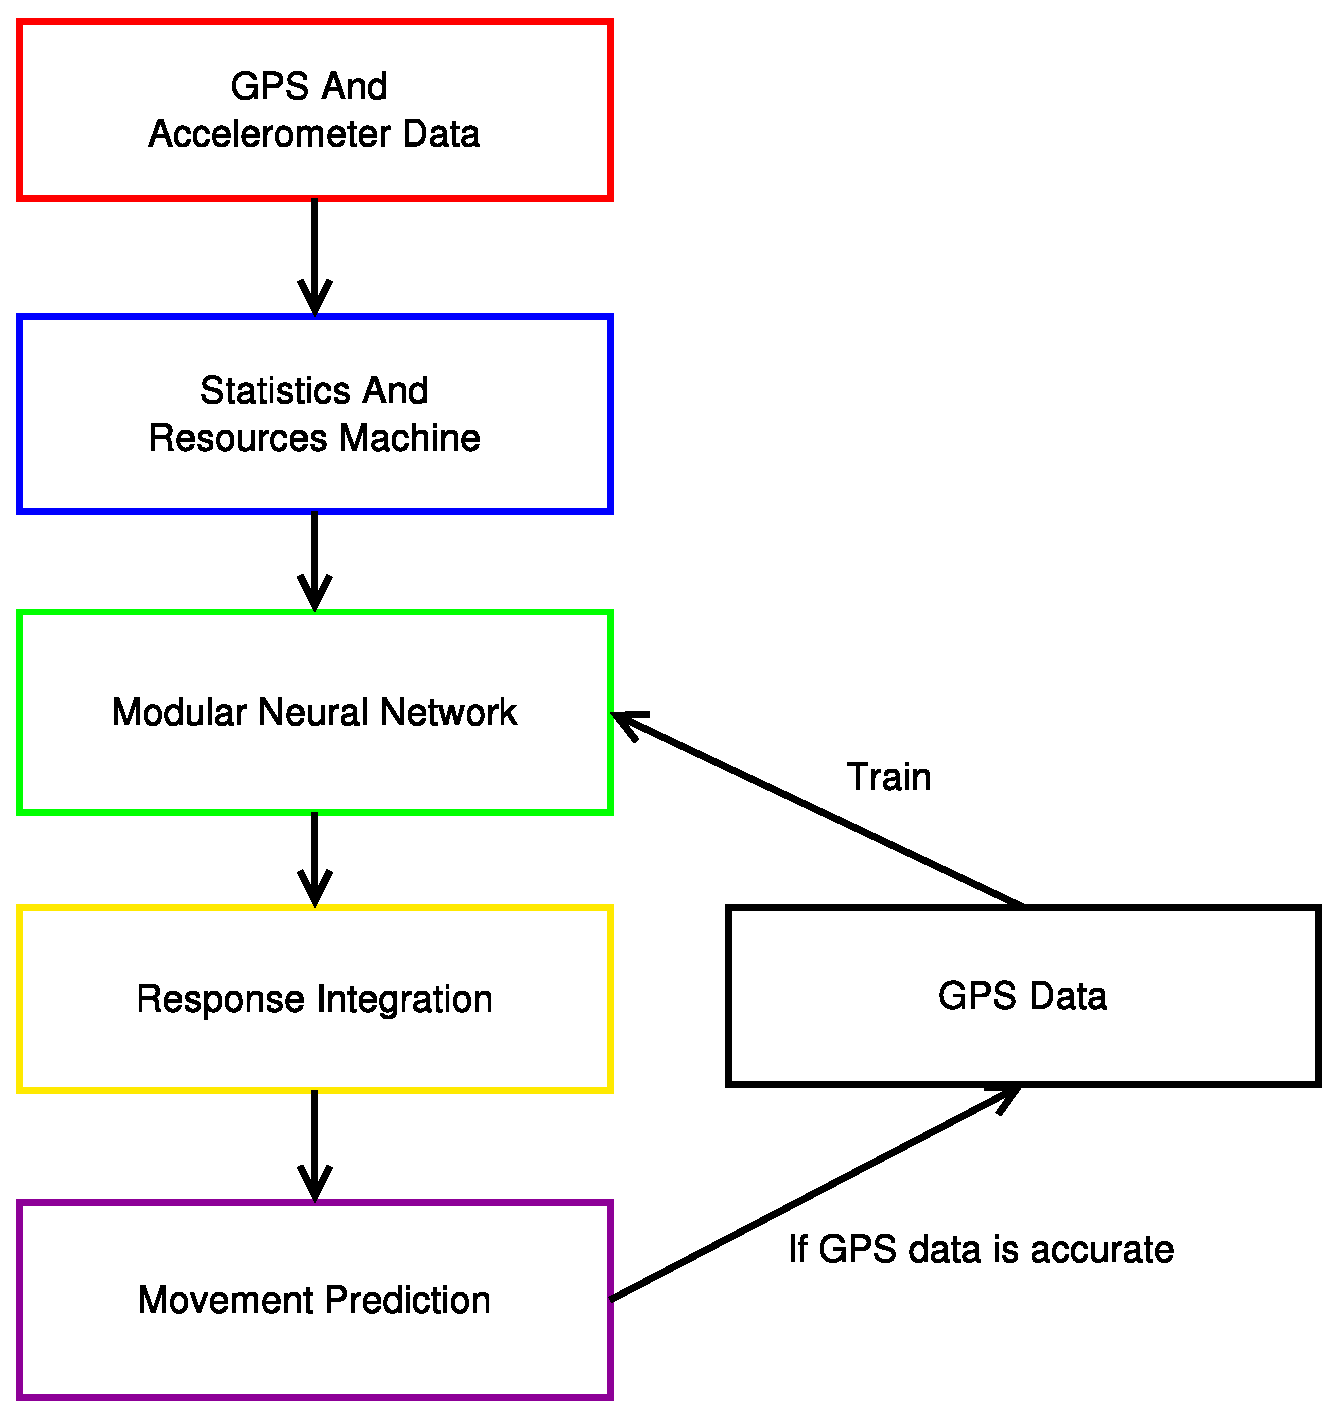
\includegraphics[scale=0.3]{../../figures/process_diagram/process}
  \end{itemize}
\end{frame}

\begin{frame}
  \frametitle{Data Collection}
  We developed an application to record accelerometer readings into
  files. For this presentation, we use a data set recorded from
  holding the phone horizontally flat while walking thirty steps in a
  straight line with a heading of $260^{\circ}$, according to the
  phone's compass.
\end{frame}

\begin{frame}
  \frametitle{Step Detection}
  $y = mx + b$ where
  \[
  m = \frac{n\sum{xy} - \left(\sum{x}\right)\left(\sum{y}\right)}
  {n\sum{(x^2)} - \left(\sum{x}\right)^2},
  \]
  \[
  b = \frac{\sum{y} - m\left(\sum{x}\right)}{n},
  \] and $n$ is the number of points.
\end{frame}

\frame[plain]{
  \begin{center}
    \scalebox{.45}{\includegraphics{z}}
  \end{center}
}

\end{document}


